\subsection{Clientseitige Architektur}

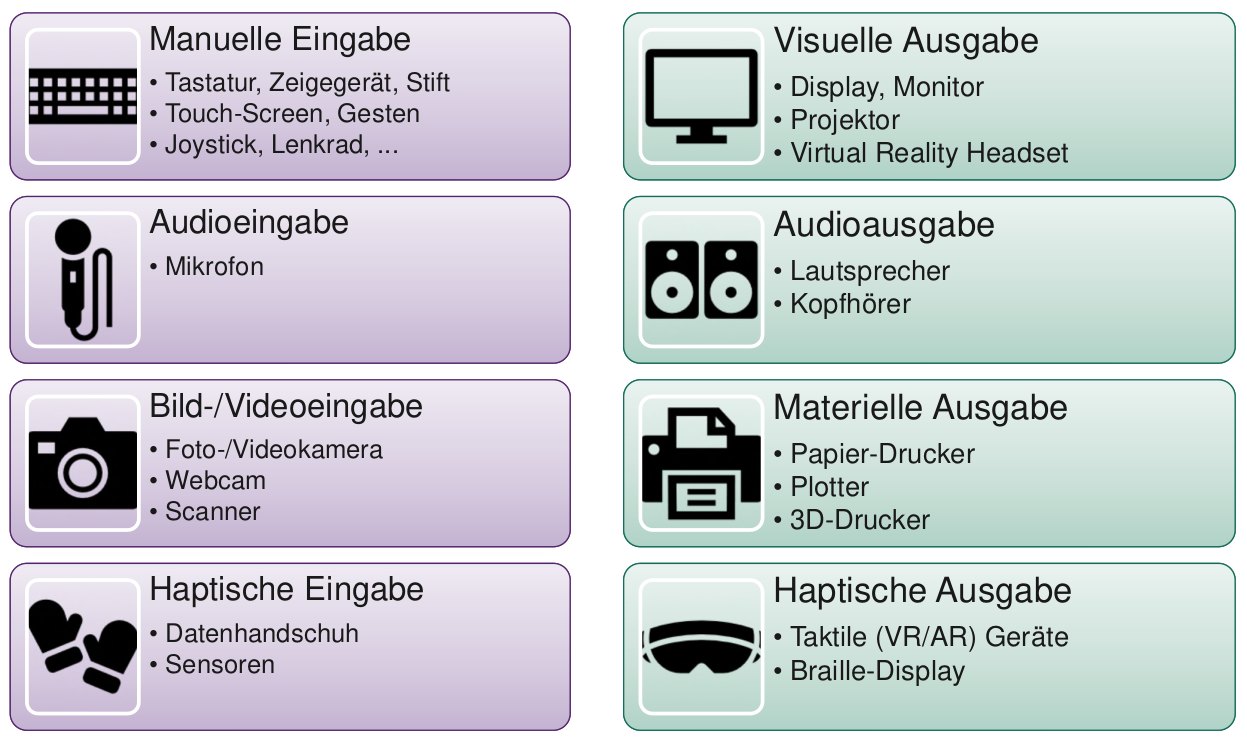
\includegraphics[width=\linewidth]{clients-hci.png}

\begin{itemize}
    \item \textcolor{blue}{Desktop Device}
    \item \textcolor{blue}{Mobile Device} Tablet, Notebook, Wearable Devices, Mobile Phone
    \item \textcolor{blue}{IoT Device} physischen Kontext (Cyber-Modell, Applikation, Analytik)
    \item \textcolor{blue}{Virtueller Device} Client zeigt nur Bild an, Verarbeitung läuft auf dem Server
\end{itemize}

\subsubsection{Client OS}

\begin{itemize}
    \item Windows
    \item Apple
    \item Linux
    \item Android
\end{itemize}

\subsubsection{Client App Technologien}

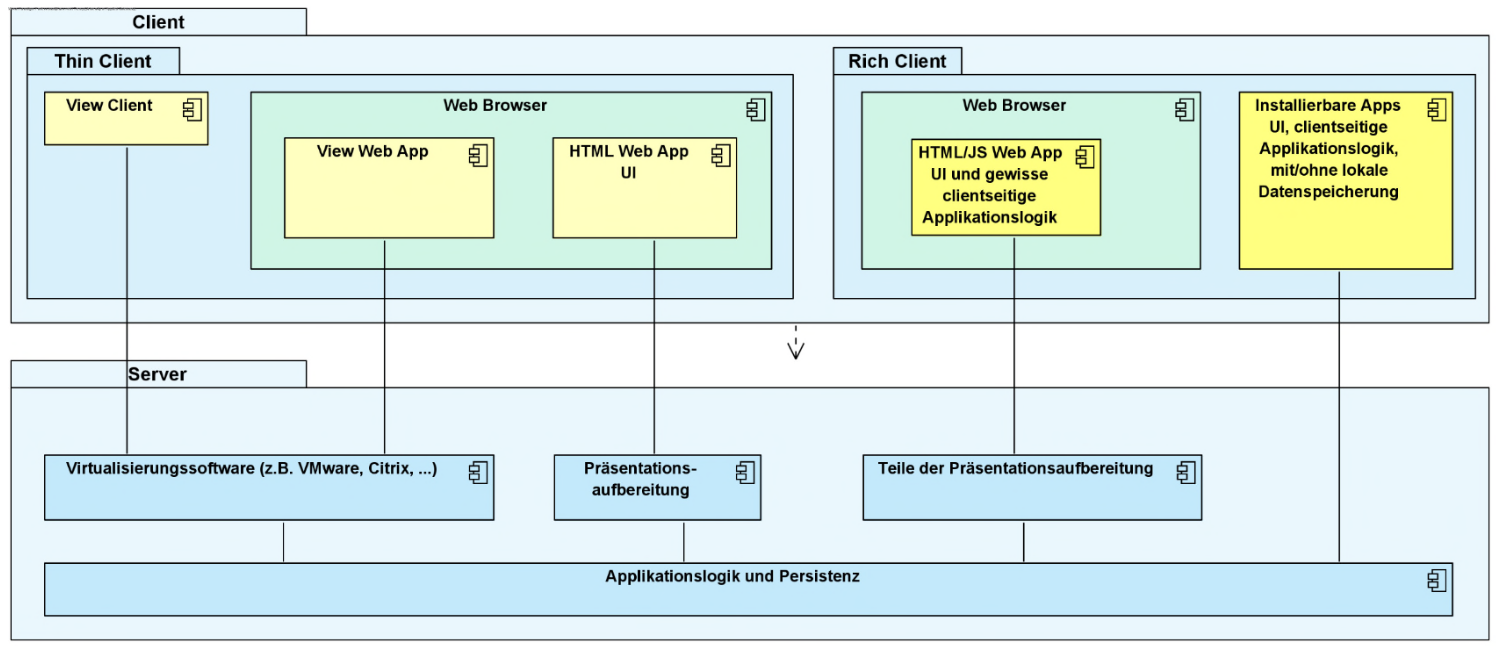
\includegraphics[width=\linewidth]{clients-devices.png} \\

\textbf{Thin Clients}

Virtuelle Desktops (VMware, Citrix), Werden im Webbrowser oder in View Clients betrieben \\

\textbf{Rich Client}

Klassische Desktop Apps, Haben meist nebst Applikationslogik, lokale Datenhaltung \\

\subsubsection{Location-L}

Location Based Services (LBS)

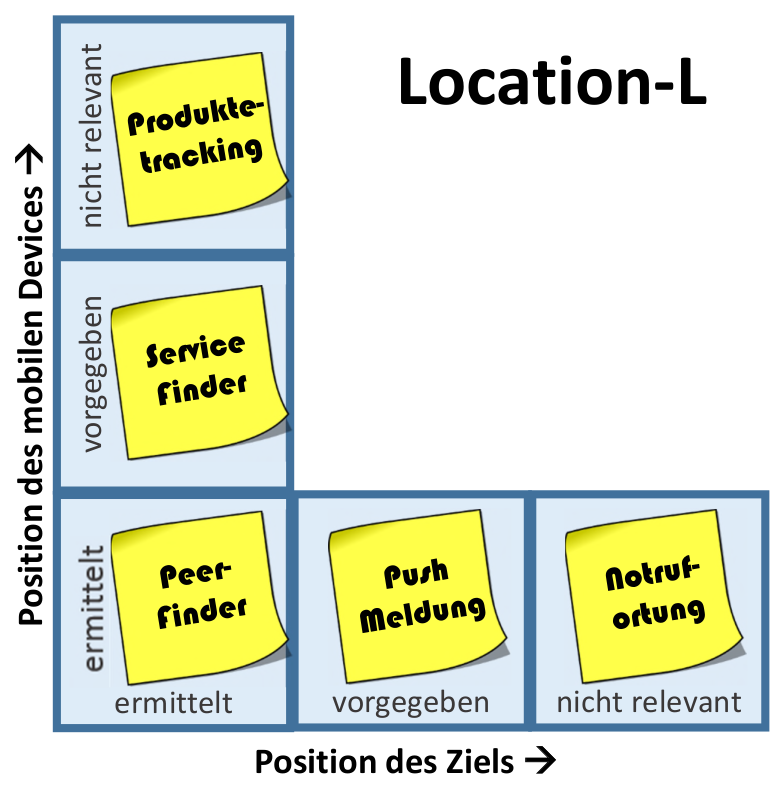
\includegraphics[width=\linewidth]{clients-l.png}
Ein Standort muss mindestens ermittelt werden!

\subsubsection{Architekturmuster/Entwurfsmuster}

\textbf{Model View Controller (MVC)}

ASP.NET oder JSF

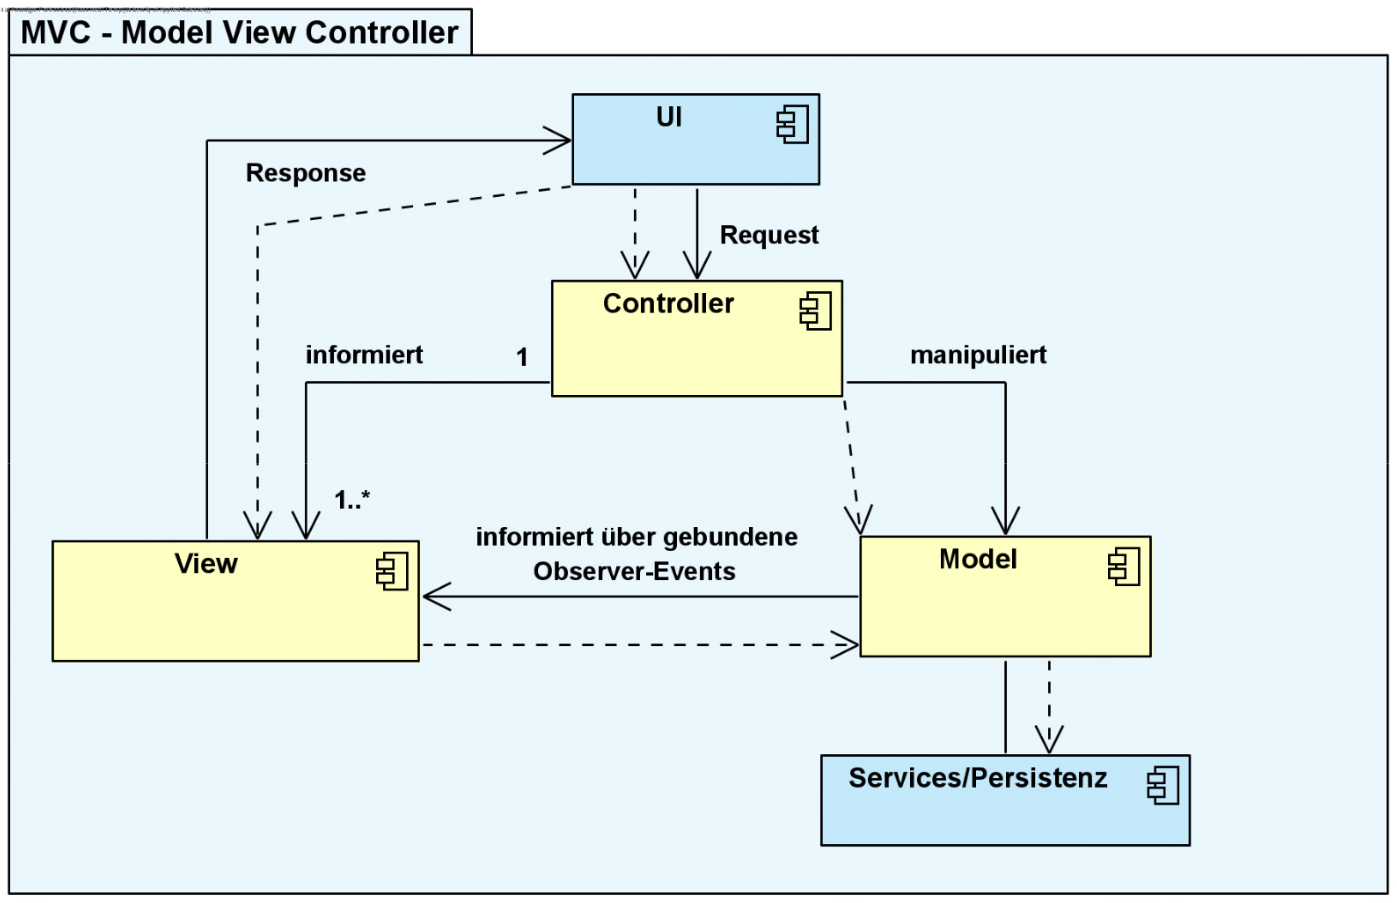
\includegraphics[width=\linewidth]{clients-mvc.png} \\


\textbf{Model View Presenter (MVP)}

bessere Testbarkeit der Komponenten und vollständiges Entkoppeln der View von dem Model. (Windows Forms)

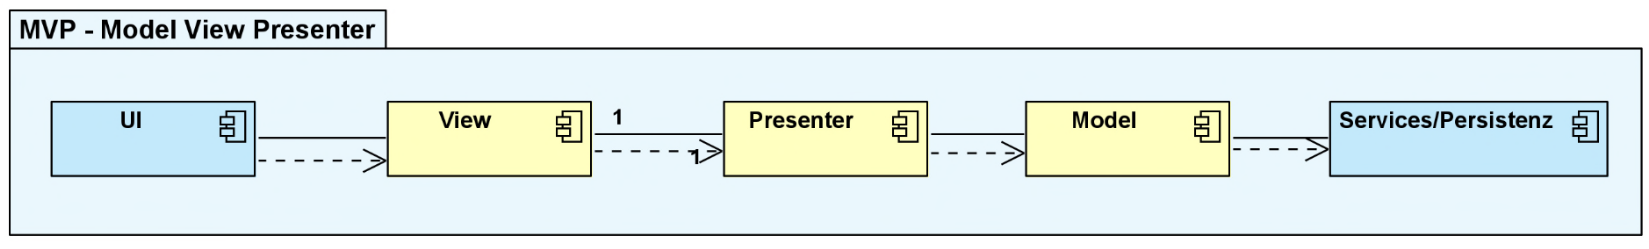
\includegraphics[width=\linewidth]{clients-mvp.png} \\

\textbf{Model View View-Model (MVVM)}

Web App

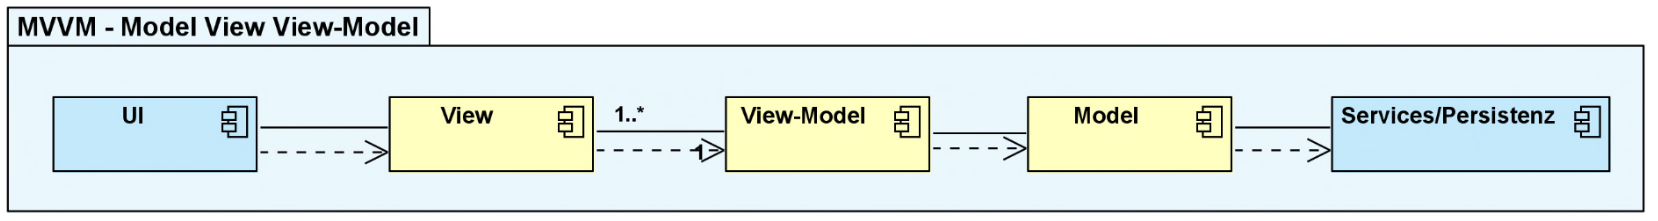
\includegraphics[width=\linewidth]{clients-mvvm.png} \\

\subsubsection{Programmiersprachtypen}

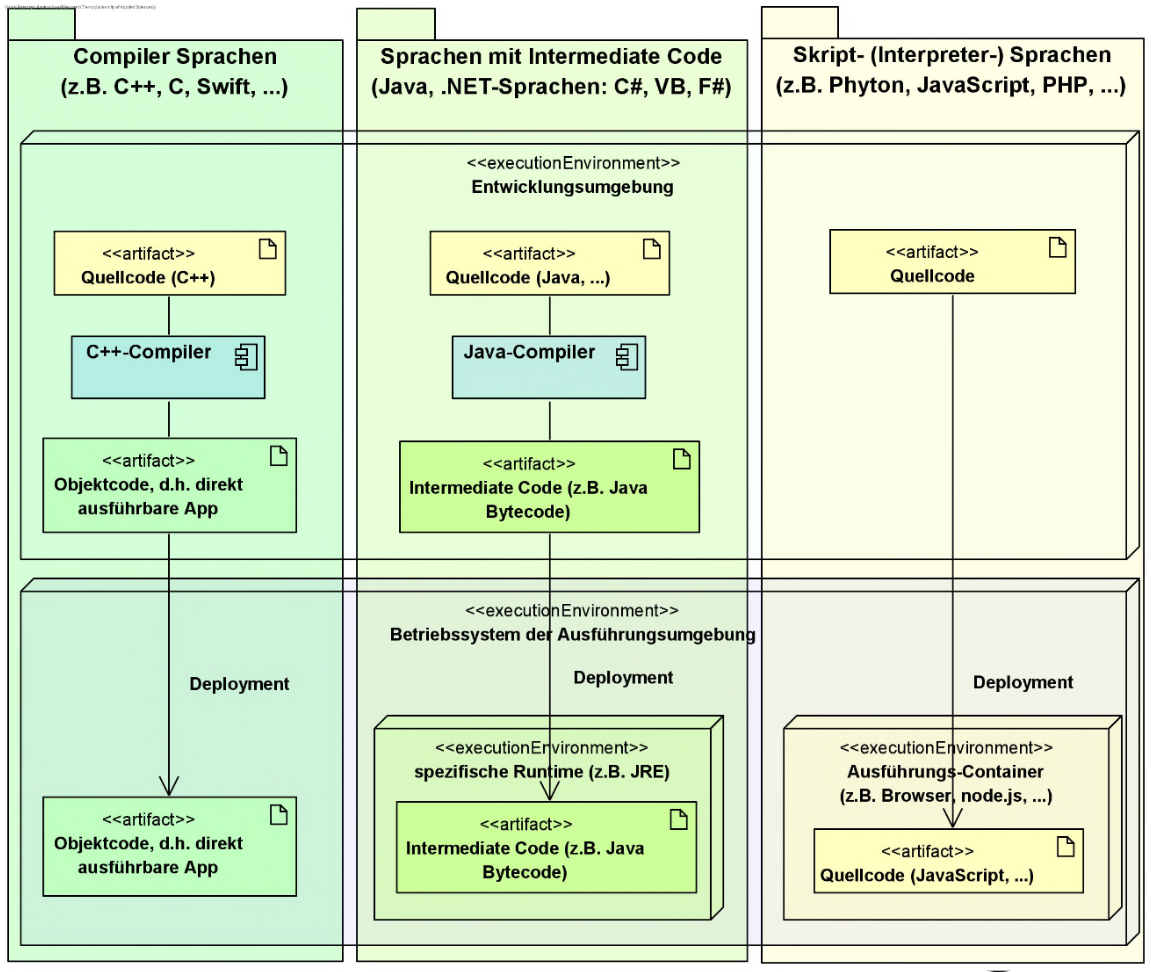
\includegraphics[width=\linewidth]{clients-programming-lang-types.png} \\

\subsubsection{Installable Client Apps}

Installable App

\textbf{Single Platform Apps} \\


\textbf{Cross Platform Apps}

\begin{itemize}
    \item Code kann gemeinsam genutzt werden
    \item Kostengünstiger
    \item Schneller Time-to-Market
\end{itemize}
\vspace{10pt}
\textbf{Multiplatform/Hybrid Apps}

Vorteile
\begin{itemize}
    \item Nutzen Devices voll aus
    \item Beste Performance
    \item UI sind voll Plattformkonform
\end{itemize}
\vspace{10pt}

Nachteile
\begin{itemize}
    \item Aufwändig
    \item Je Plattform ein eigenes Entwicklerteam
\end{itemize}

\subsubsection{Client WebApps}

Ausführung im Web Browser

\textbf{HTML5 mit/ohne JS} \\

\textbf{SPA}

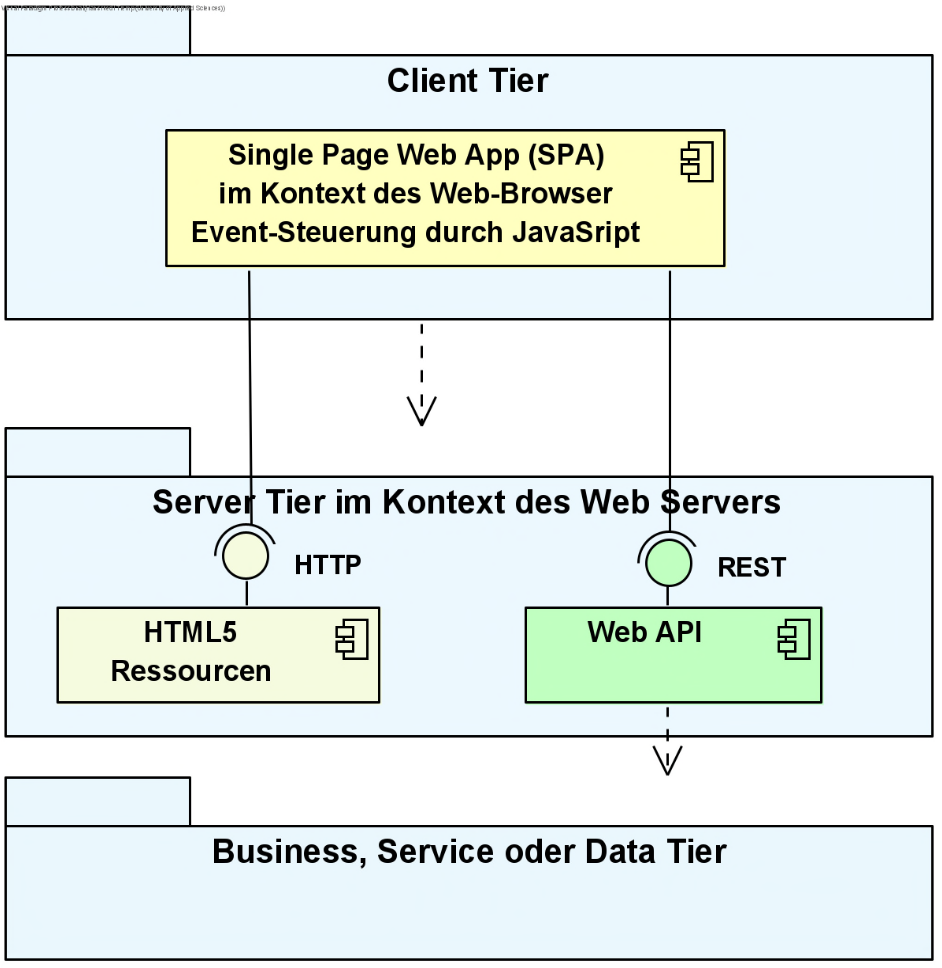
\includegraphics[width=\linewidth]{clients-spa.png} \\

\textbf{PWA}

Webbrowser startet als unsichtbarer Container anhand der Informationen im Manifest, Requests erfolgen über Service Worker (Netzwerk vorhanden: Request beim Server vornehmen und Ergebnis im Cache aktualisieren, Netzwerk nicht vorhanden: Werte aus dem Cache auslesen)

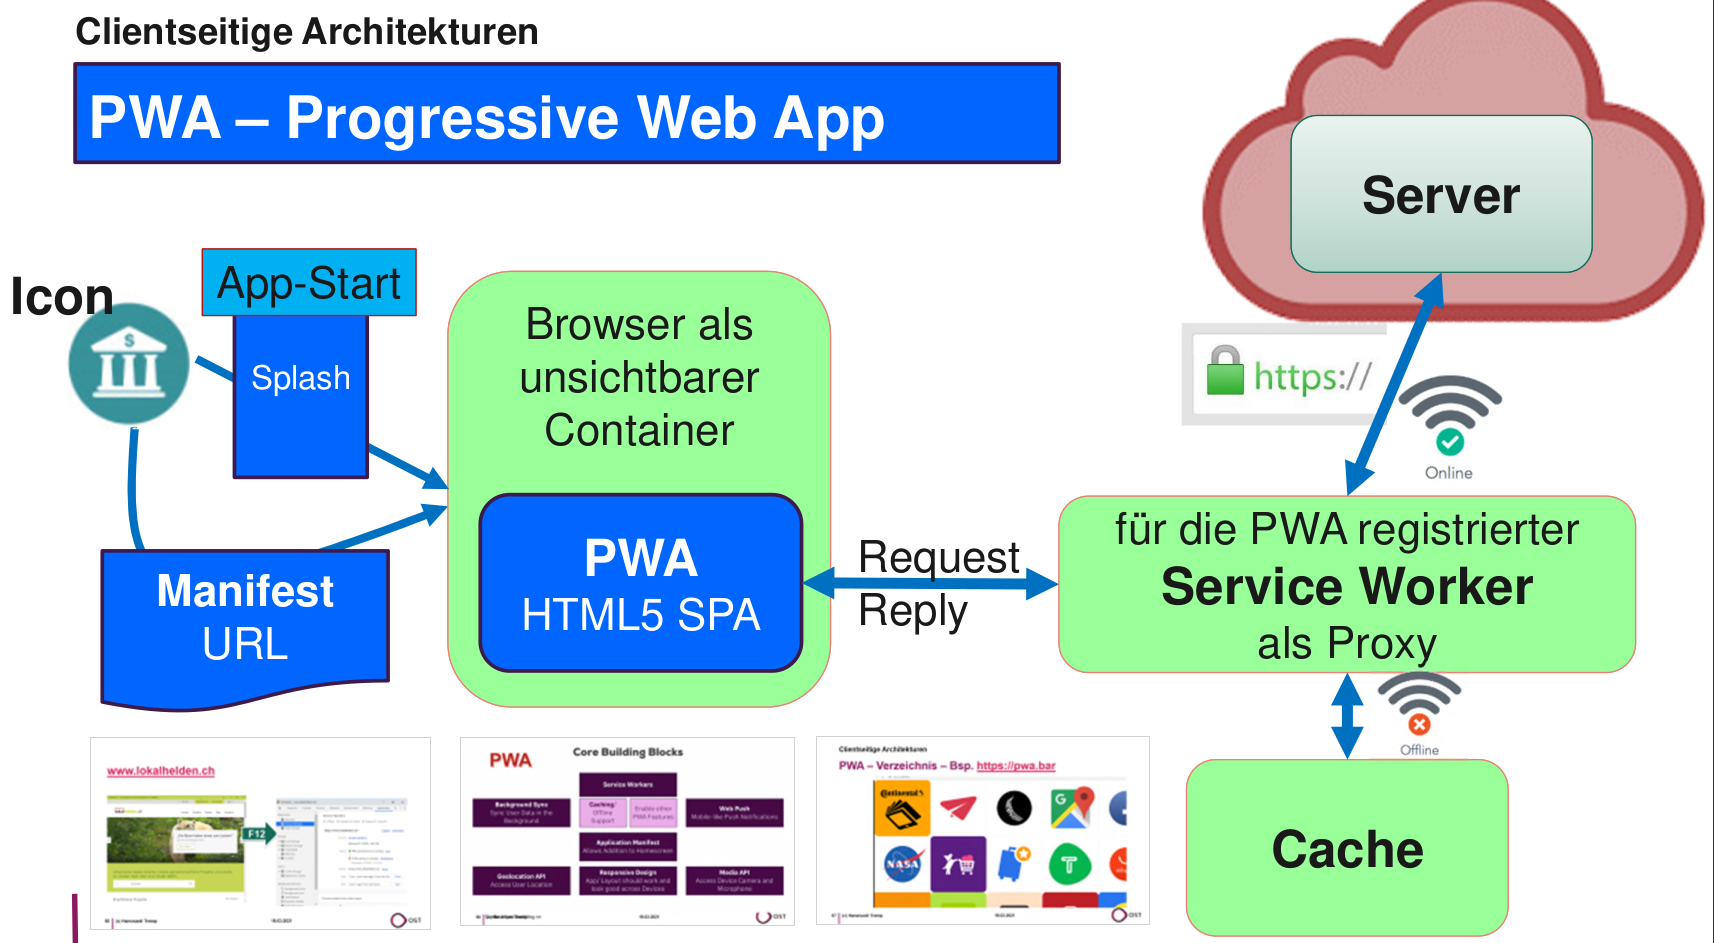
\includegraphics[width=\linewidth]{clients-pwa.png} \\

\textbf{Serverframework ASP.NET Core}

ASP – Active Server Page mit MVC Muster, Kestrel fungiert als Webserver

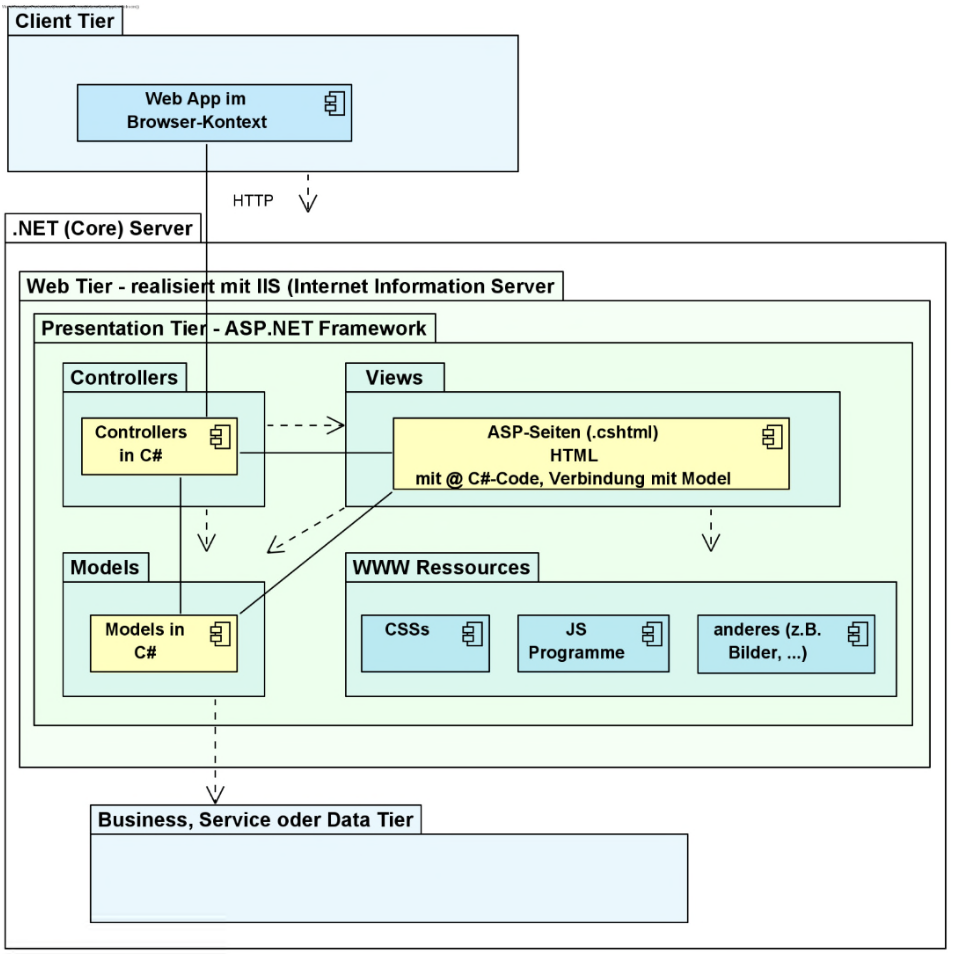
\includegraphics[width=\linewidth]{clients-asp.png} \\

\textbf{Serverframework Java EE}

JSF – Java Server Faces, zusätzlich Frameworks wie z.B. Spring usw., EJBs enthalten Business-Logik und die Connection zur DB

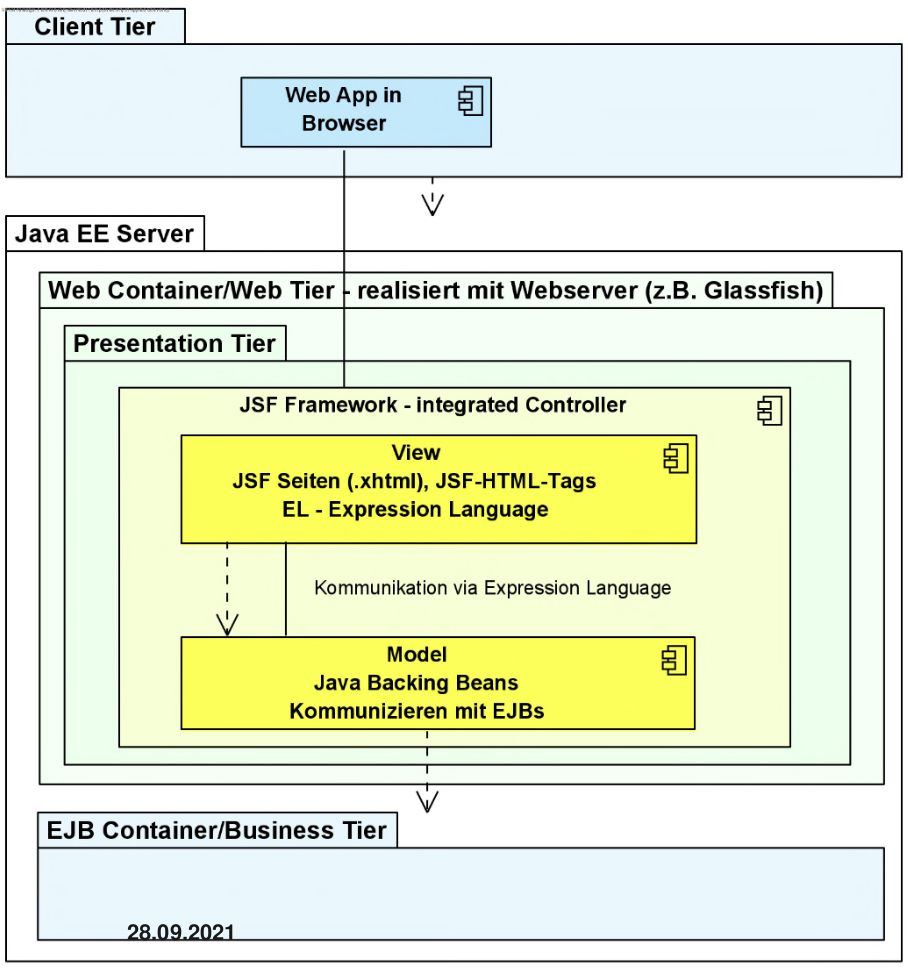
\includegraphics[width=\linewidth]{clients-java.png}

\subsubsection{Makroarchitektur}

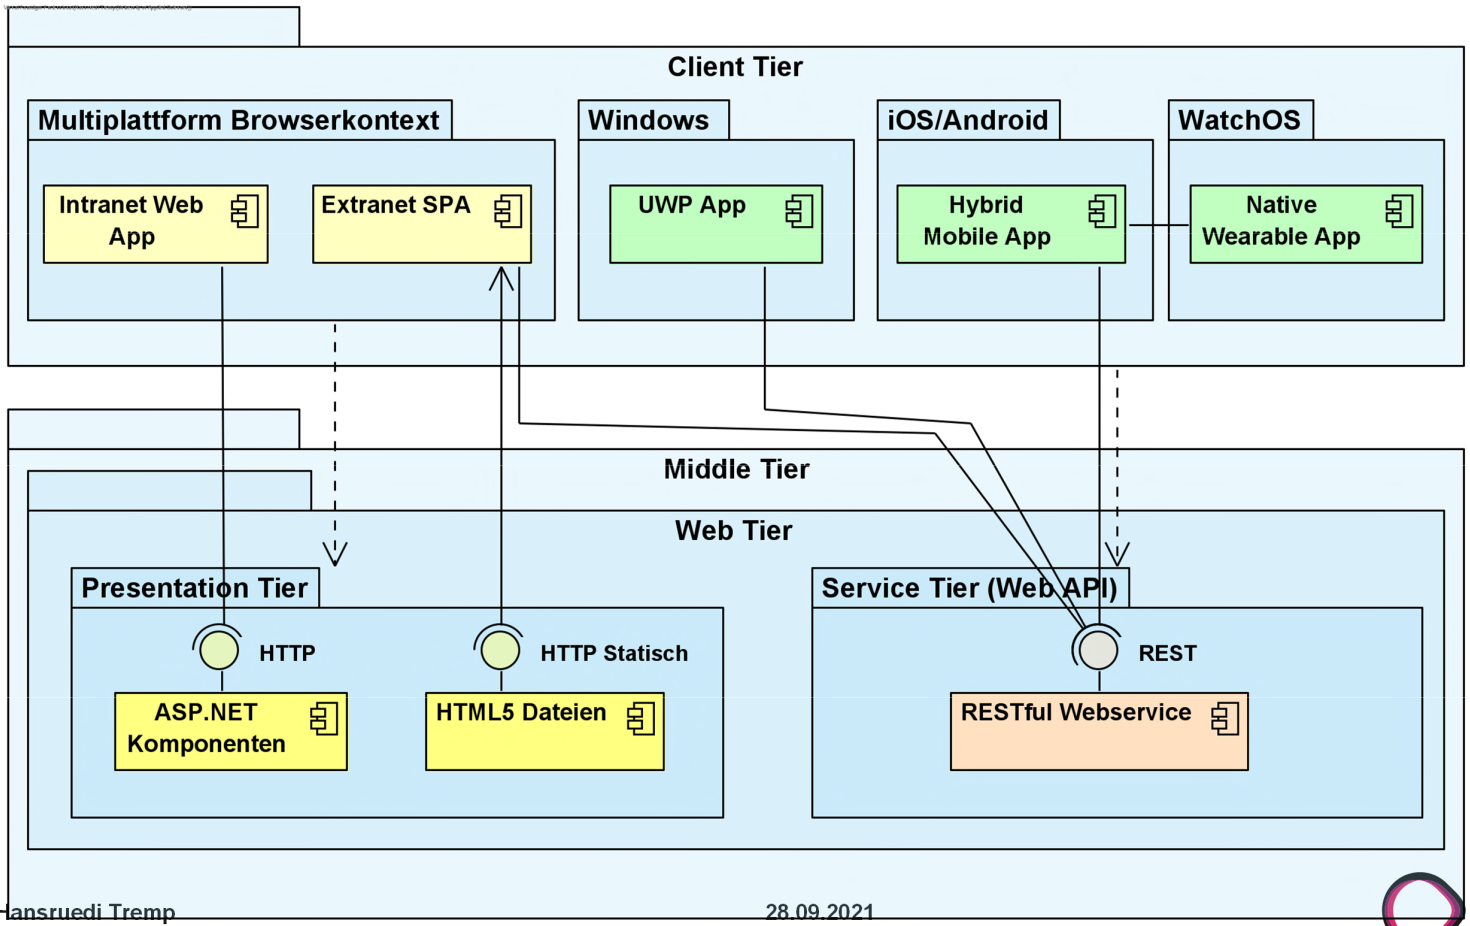
\includegraphics[width=\linewidth]{clients-macro-arch.png} \\

\textbf{Strukturierungsoptionen für das GUI}

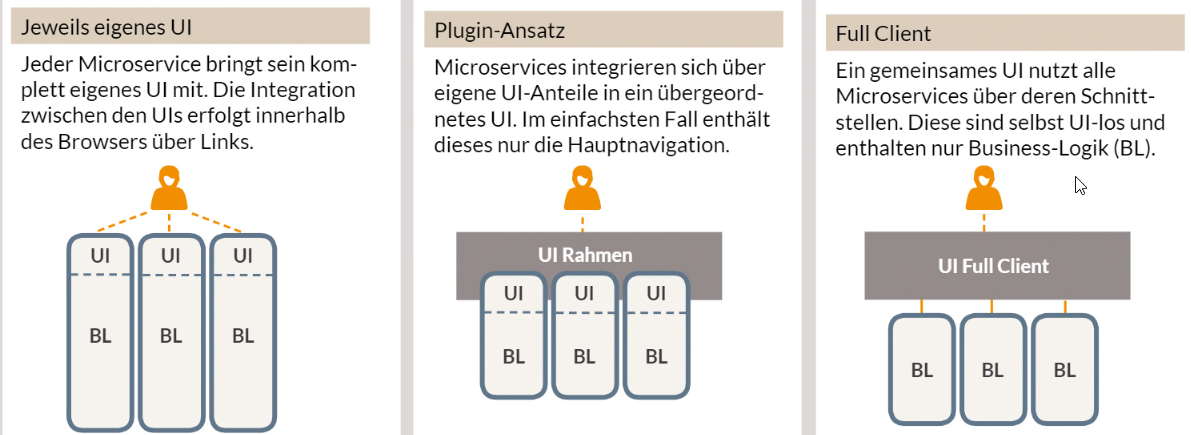
\includegraphics[width=\linewidth]{clients-gui-structures.png}

\subsubsection{Prüfungsfragen}

\begin{itemize}
    \item Was ist DaaS, aus welchen Komponenten besteht deren Infrastruktur und welche Vorteile ergeben sich für den Anwender sowie den Betreiber der IT? \\
    \textcolor{blue}{Device as a Service. Sind Virtuelle Desktops. Faster deployment and decommissioning of active end users. Reduced downtime for IT support. Cost savings. Increased Device flexibility, Enhanced Security}
    \item Wie funktioniert AJAX und welcher Nutzen ergibt sich für die UX? \\
    \textcolor{blue}{Seiten können dynamisch asynchron Nachgeladen werden.}
    \item Was ist der Unterschied zwischen AR und VR? \\
    \textcolor{blue}{AR verwendet real-world Settings und VR ist komplett virtuell}
    \item Welche drei Sprachen kommen in einer Web App primär zur Anwendung und welche Funktionen übernehmen diese? \\
    \textcolor{blue}{HTML, CSS und JavaScript}
\end{itemize}
